\chapter{User Manual}

\startcontents[manual]
\printcontents[manual]{}{1}{}

\section{Introduction}
\subsection{Purpose of the system}
The purpose of the application is to store data of members and parents and to store details of invoices, with the data is both cases being easily but securely accessed. The application has the ability to view, add, edit and delete data in a database, with  and ordering, sorting and basic validation capabilities.

\subsection{Intended audience}
The intended audience for this application is scout leaders of the Fordham Cub Scout group, however other scout groups could use the system.

\section{Installation}

\subsection{Software}
As the program is an executable file, no extra software is needed to run the program. However, the program is downloaded as a compressed file, so an extractor is needed to unpack the files, such as WinRar.

\subsection{Hardware}
\begin{itemize}
	\item A mouse and keyboard for input
	\item A computer for processing
	\item A monitor for visual output
	\item A storage medium to download to and to store the database
	\item A printer to print the invoices
\end{itemize}

\subsection{Operating System}
The program has been tested on a windows 7 and windows 8 computer 64-bit computer and was compiled by a windows 8 64-bit computer. The tutorial uses windows 8, however windows 7 will be very similar.

\subsection{Downloading the file}

1. Download the executable file from this location: \url{https://www.dropbox.com/s/jsye4dmhyme3mk2/ScoutingProgramCoursework.rar?dl=0}

\begin{figure}[H]
	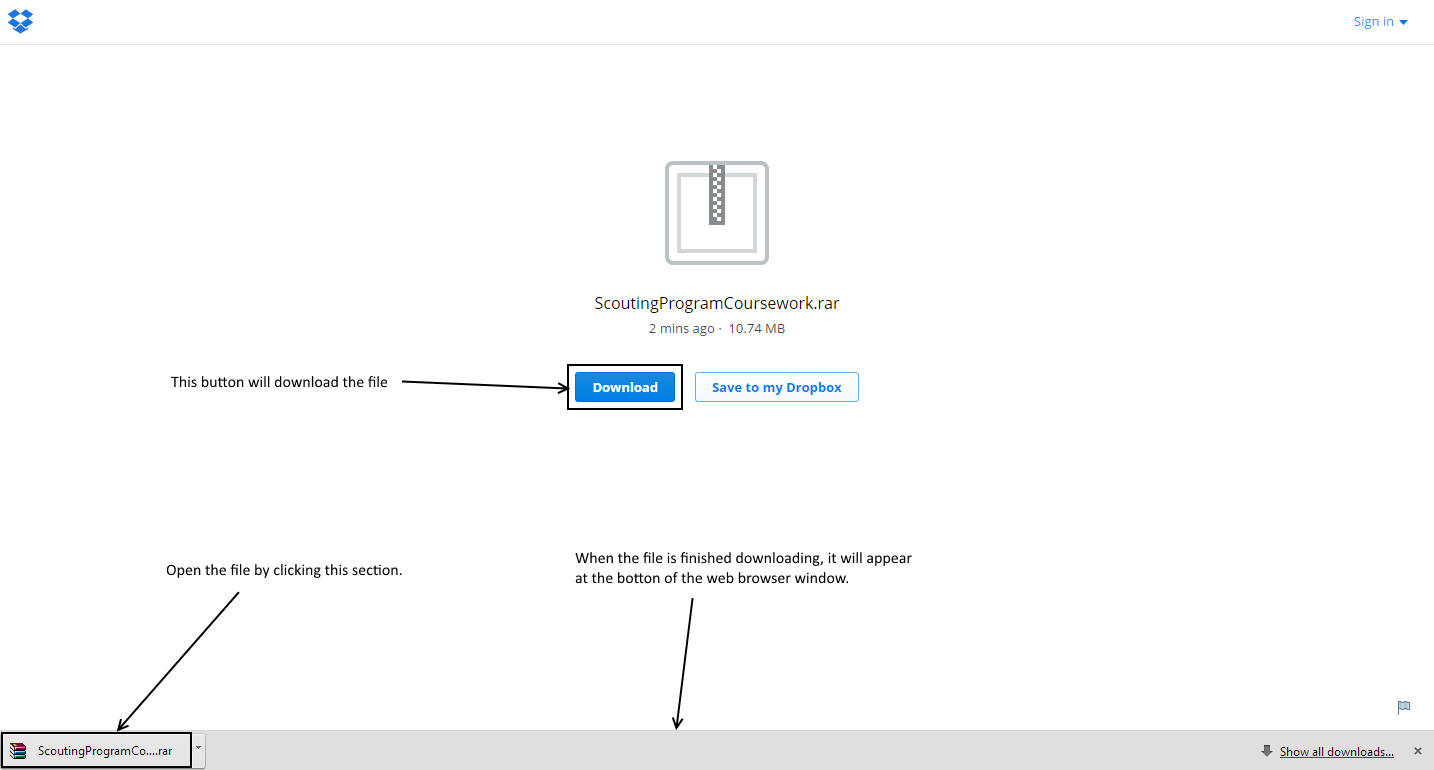
\includegraphics[width=\textwidth]{./Manual/Images/DownloadingFile.png}
	\caption{Downloading File} \label{fig:download_file}
\end{figure}

Note that if you have a dropbox account or are using a web browser other than google chrome the screen may be slightly different.


2. Extract the folder in the compressed file to a location of your choosing.

\begin{figure}[H]
	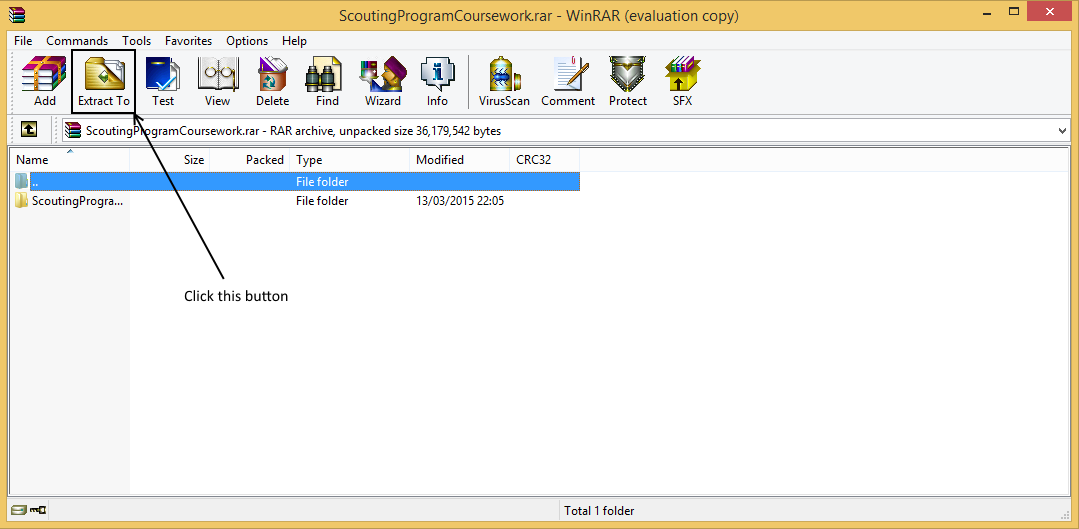
\includegraphics[width=\textwidth]{./Manual/Images/Extracting1.png}
	\caption{Extracting File} \label{fig:extracting_file_1}
\end{figure}

\begin{figure}[H]
	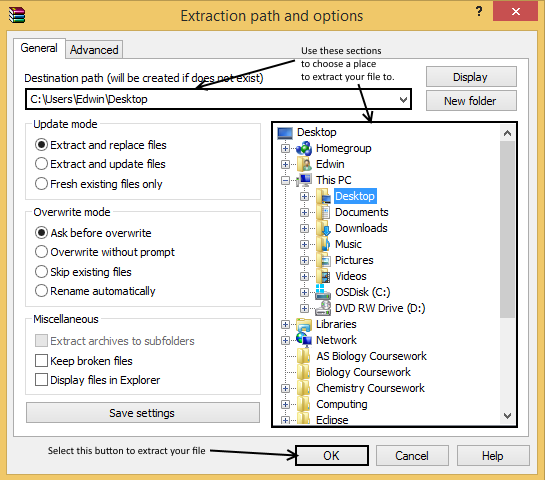
\includegraphics[width=\textwidth]{./Manual/Images/Extracting2.png}
	\caption{Extracting File} \label{fig:extracting_file_2}
\end{figure}

Note that if you are not using WinRar then the method may be slightly different.

3. If desired, you can create a shortcut to the program by right clicking on the .exe and selecting 'create new shortcut'. Then drag the shortcut onto the desktop.

\begin{figure}[H]
	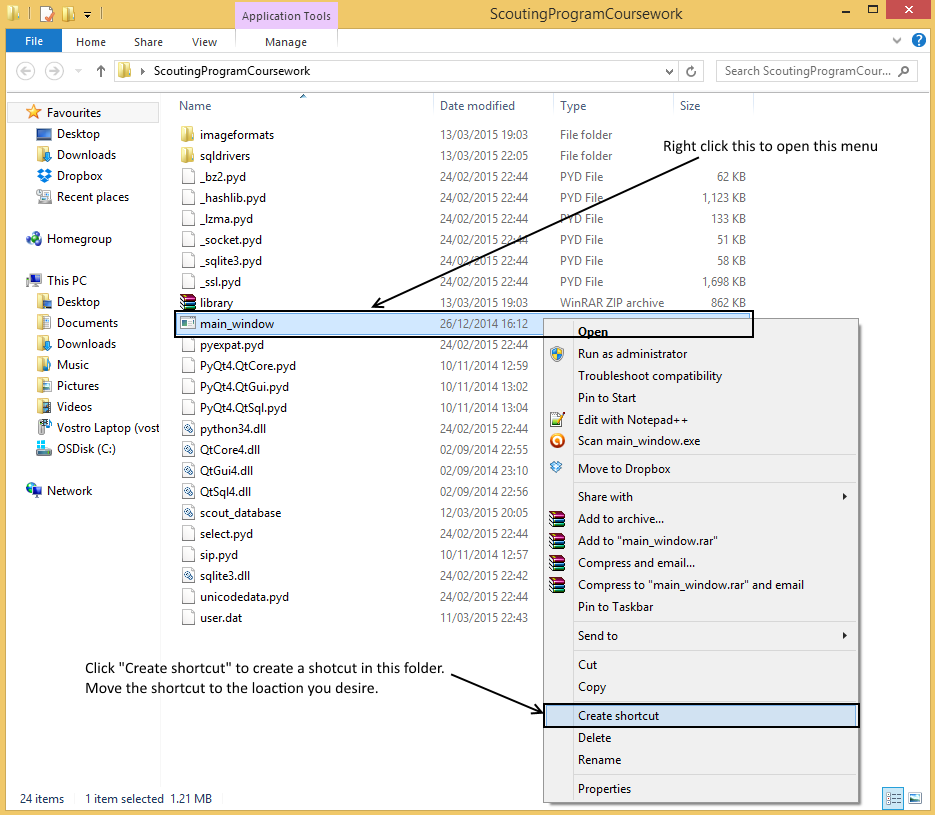
\includegraphics[width=\textwidth]{./Manual/Images/CreateShortcut.png}
	\caption{Create Shortcut} \label{fig:create_shortcut}
\end{figure}

\subsection{Running the file}

Simply open the extracted folder and run the .exe to run the program, or use the shortcut if you created one.

\begin{figure}[H]
	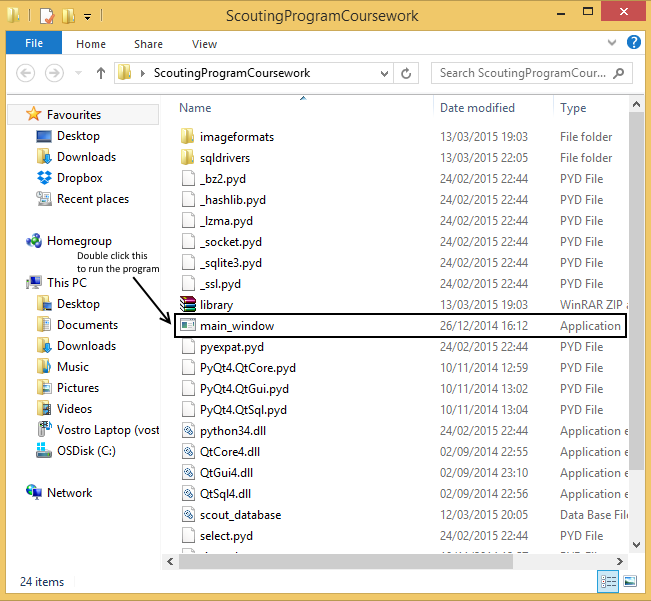
\includegraphics[width=\textwidth]{./Manual/Images/RunProgram.png}
	\caption{Run Program} \label{fig:run_program}
\end{figure}

\section{Tutorial}

\subsection{Introduction}
This tutorial is designed to take you through the steps to using all the functions of the program. To do this I will use images of the program in action and descriptions of those images.

\subsection{Assumptions}
This tutorial assumes you know how a database works.

\subsection{Tutorial Questions}

\begin{center}
	\begin{longtable}{|p{2cm}|p{4cm}|p{4cm}|}
		\hline
		\textbf{Section Number}  &  \textbf{Question}  &  \textbf{Page number}  \\ \hline
		5.3.3 & How do I log in? & \pageref{login_screen} \\ \hline
		5.3.3 & How do I show members? & \pageref{show_member} \\ \hline
		5.3.3 & How do I show parents? & \pageref{show_parent} \\ \hline
		5.3.3 & How do I show invoices? & \pageref{show_invoice} \\ \hline
		5.3.3 & How do I order data? & \pageref{show_member} \\ \hline
		5.3.3 & How do I search for data? & \pageref{show_member} \\ \hline
		5.3.4 & How is a new member added? & \pageref{add_member} \\ \hline
		5.3.5 & How is a new parent added? & \pageref{add_member} \\ \hline
		5.3.6 & How is a new invoice added? & \pageref{add_member} \\ \hline
		5.3.7 & How is a member edited? & \pageref{edit_member} \\ \hline
		5.3.8 & How is a parent edited? & \pageref{edit_member} \\ \hline
		5.3.9 & How is an invoice edited?  & \pageref{edit_member} \\ \hline
		5.3.7 & How is a member deleted? & \pageref{delete_member} \\ \hline
		5.3.8 & How is a parent deleted? & \pageref{delete_member} \\ \hline
		5.3.9 & How is an invoice deleted?  & \pageref{delete_member} \\ \hline
		5.3.10 & How do I show which invoices have not been paid? & \pageref{report_invoice} \\ \hline
	\end{longtable}
\end{center}

\subsubsection{How do I log in?}
\label{login_screen}

\begin{enumerate}
	\item This screen is shown when the program is run.
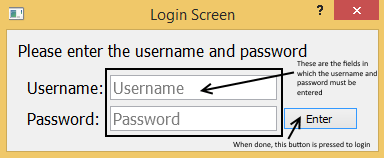
\includegraphics[width=\textwidth]{./Manual/Images/Login1.png}
	\item Enter the correct username and password. By default, the username is ''User'' and the password is ''Password''.
	\item If incorrect this window will be shown. Press close to return to the login screen.
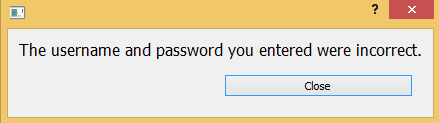
\includegraphics[width=\textwidth]{./Manual/Images/Login3.png}
	\item If correct you will be taken to the main window.
\end{enumerate}


\subsubsection{How do I show members?}
\label{show_member}

\begin{enumerate}
	\item Click the Display Member button on the menu bar in the drop down menu under Display Database or directly on the tool bar.
	\item To order the members, select a method of ordering from the drop down menu.
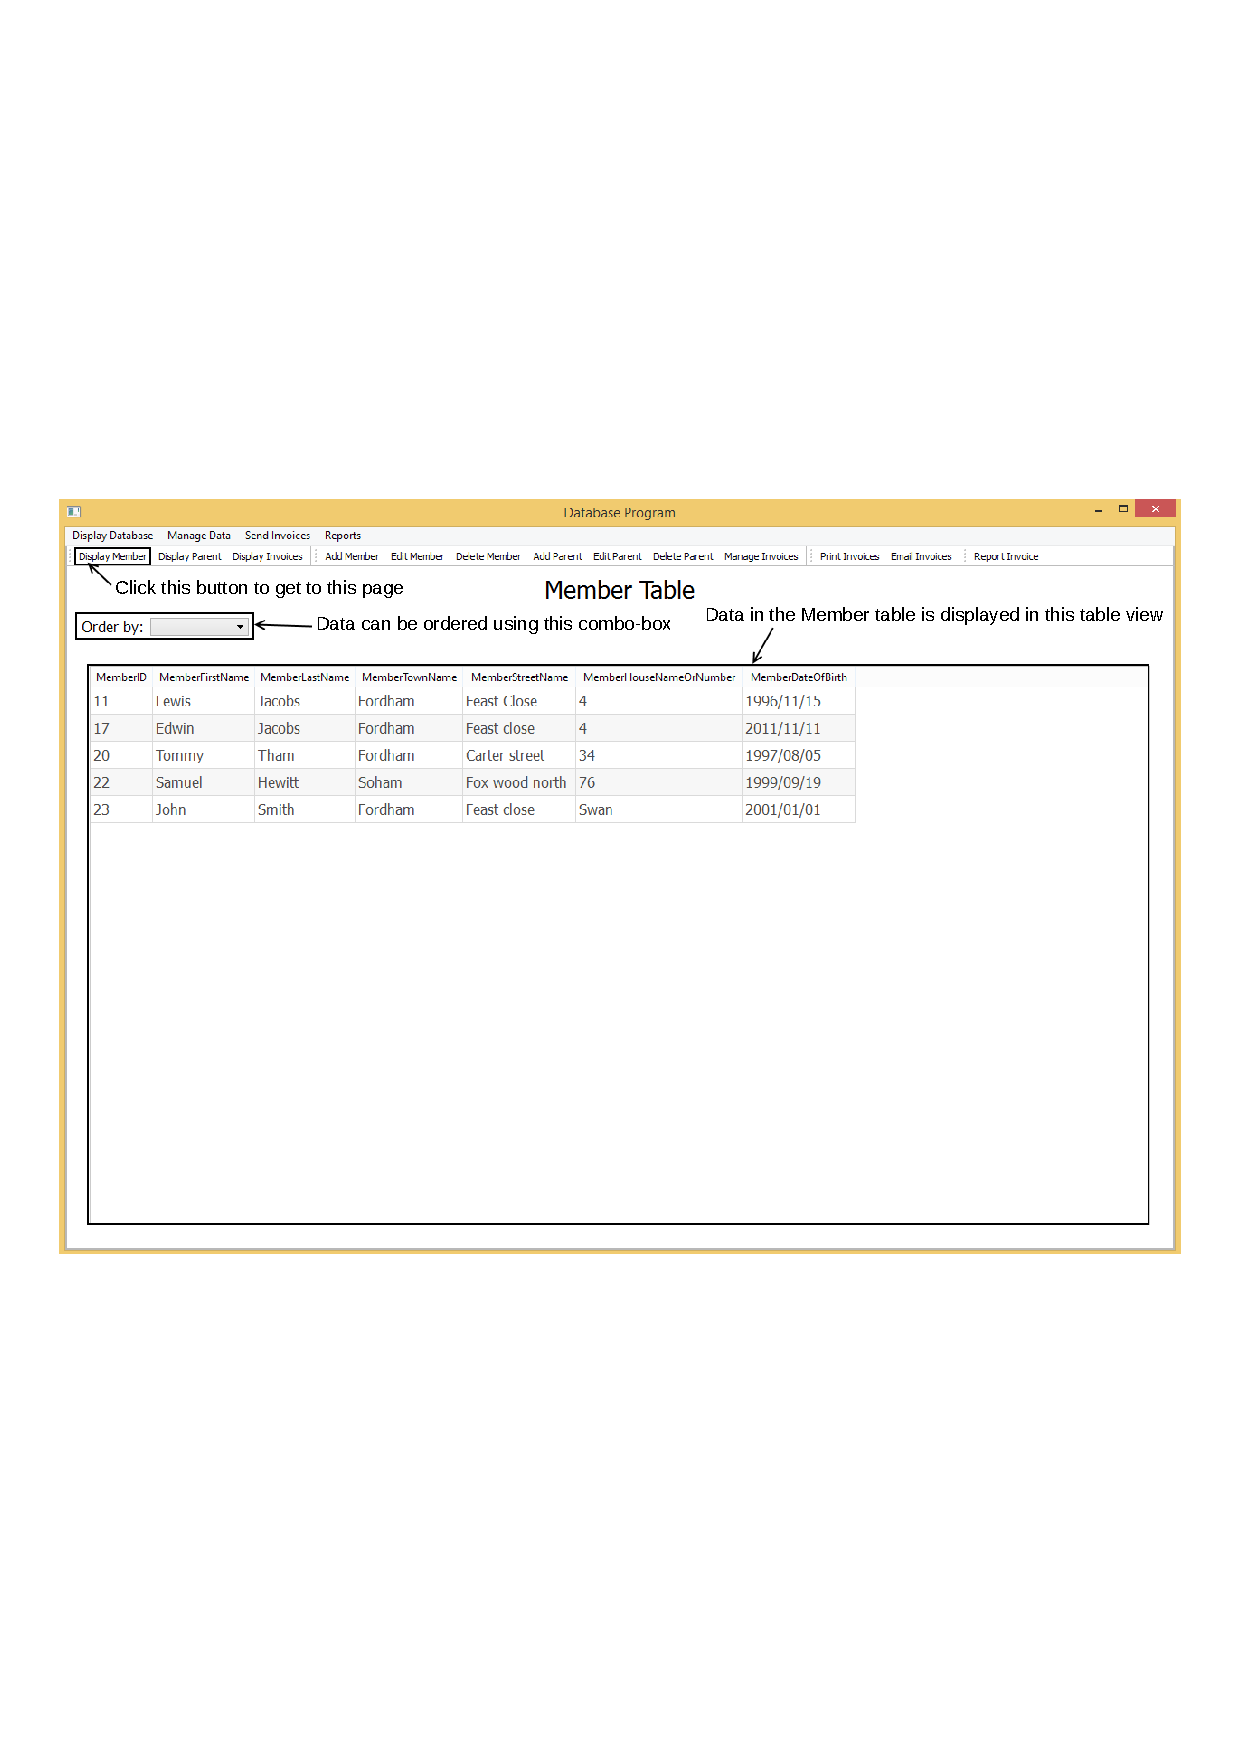
\includegraphics[width=\textwidth]{./Manual/Images/ShowMember.pdf}
\end{enumerate}


\subsubsection{How do I show parents?}
\label{show_parent}

\begin{enumerate}
	\item Click the Display Parent button on the menu bar in the drop down menu under Display Database or directly on the tool bar.
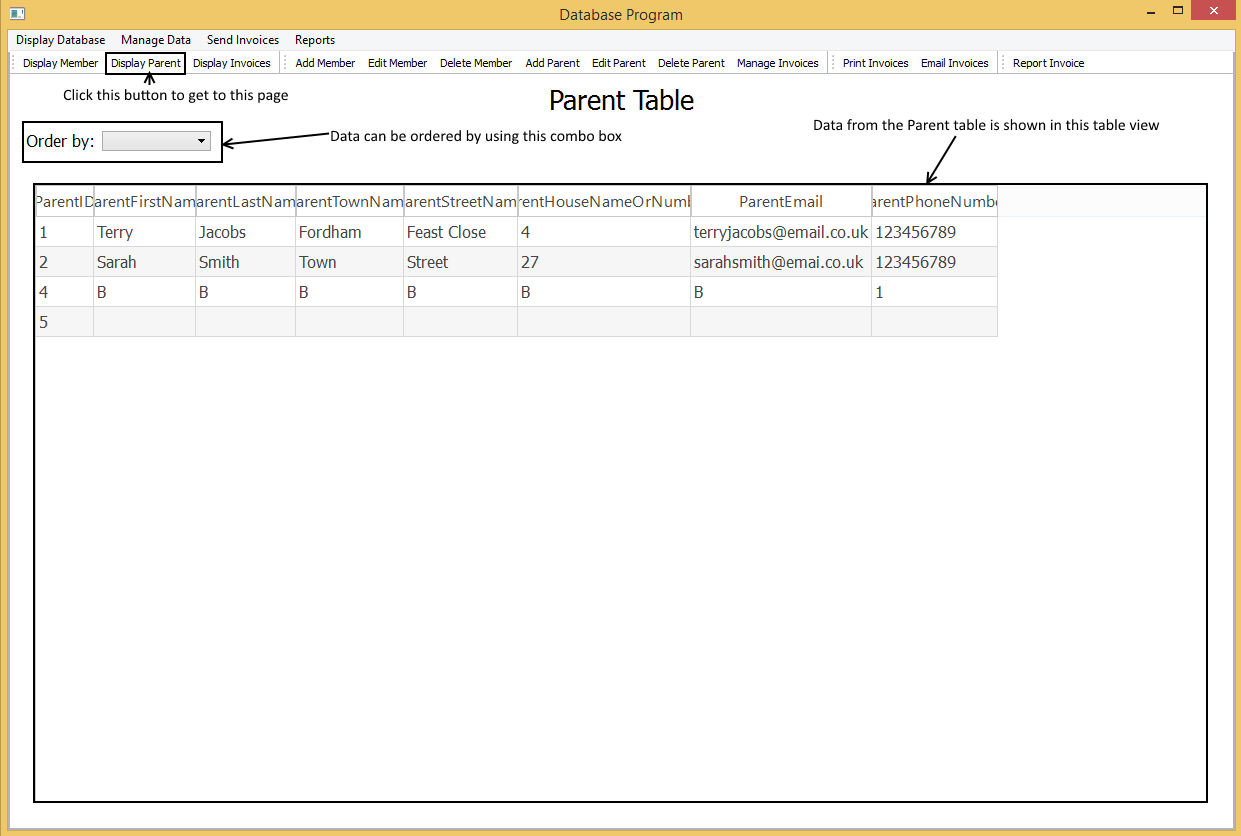
\includegraphics[width=\textwidth]{./Manual/Images/ShowParent.png}
	\item To order the parents, select a method of ordering from the drop down menu.
\end{enumerate}


\subsubsection{How do I show invoices?}
\label{show_invoice}

\begin{enumerate}
	\item Click the Display Invoices button on the menu bar in the drop down menu under Display Database or directly on the tool bar.
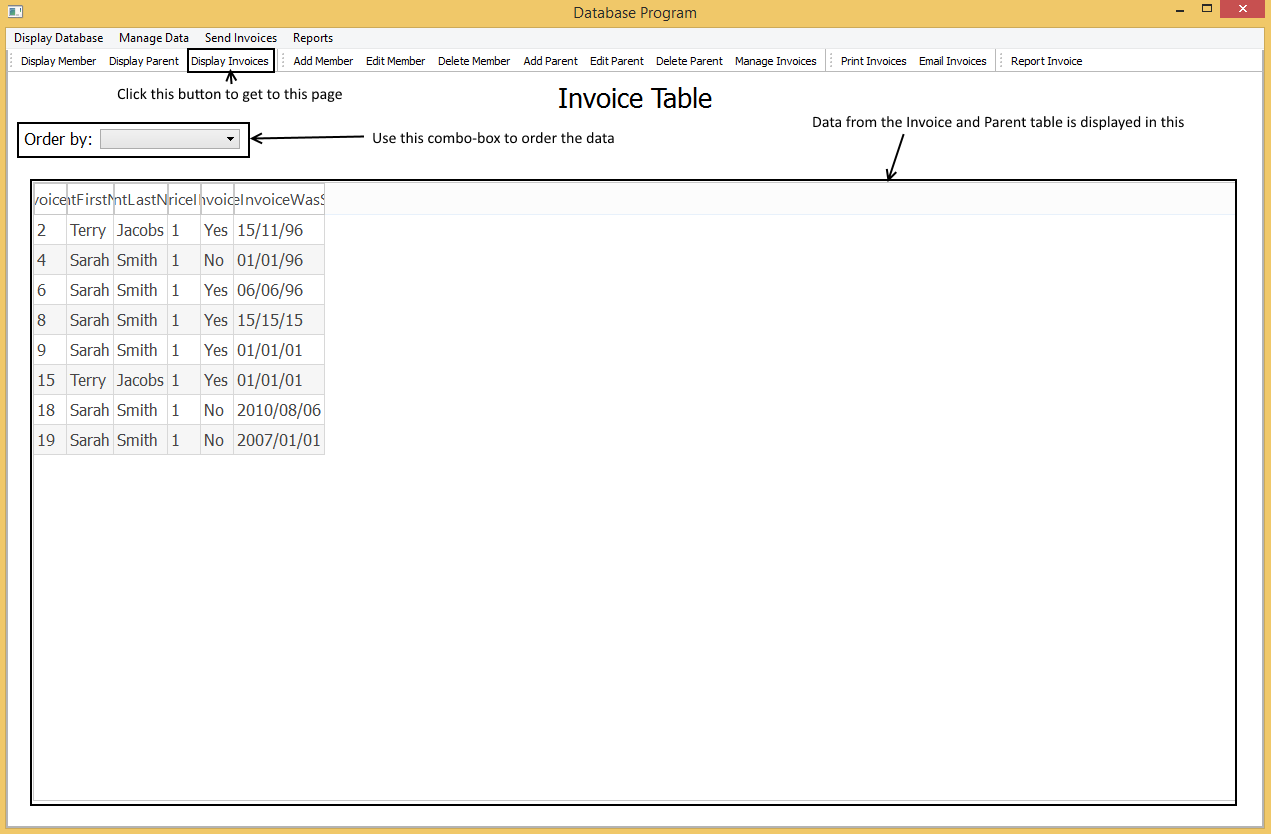
\includegraphics[width=\textwidth]{./Manual/Images/ShowInvoice.png}
	\item To order the invoices, select a method of ordering from the drop down menu.
\end{enumerate}


\subsubsection{How is a new member added?}
\label{add_member}

\begin{enumerate}
	\item Click the Add Member button on the menu bar in the drop down menu under Manage Data or directly on the tool bar.
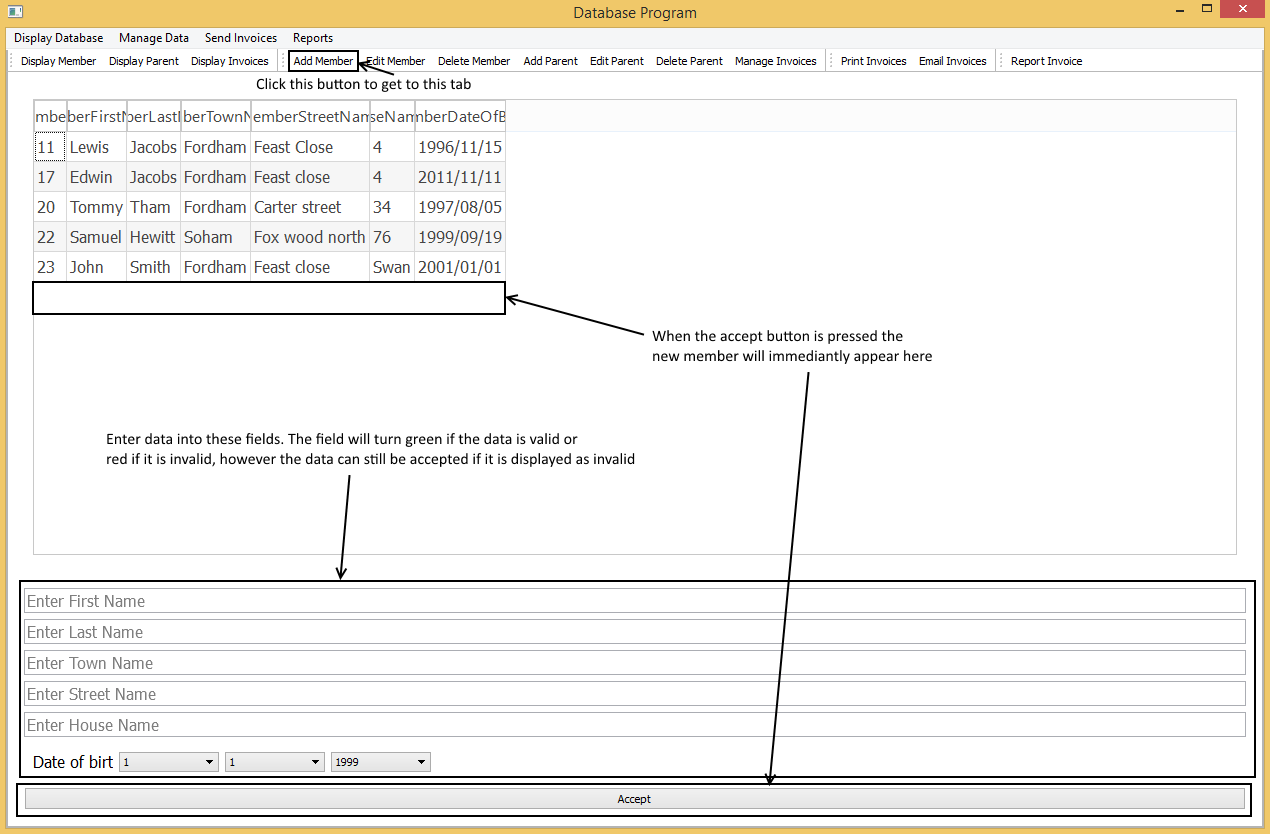
\includegraphics[width=\textwidth]{./Manual/Images/AddMember1.png}
	\item To add a member, enter the data of the member to be added in the fields at the bottom.
	\item When done, press the accept button. The new member should immediatly appear in the table.
\end{enumerate}

\subsubsection{How is a member edited?}
\label{edit_member}

\begin{enumerate}
	\item Click the Edit Member button on the menu bar in the drop down menu under Manage Data or directly on the tool bar.
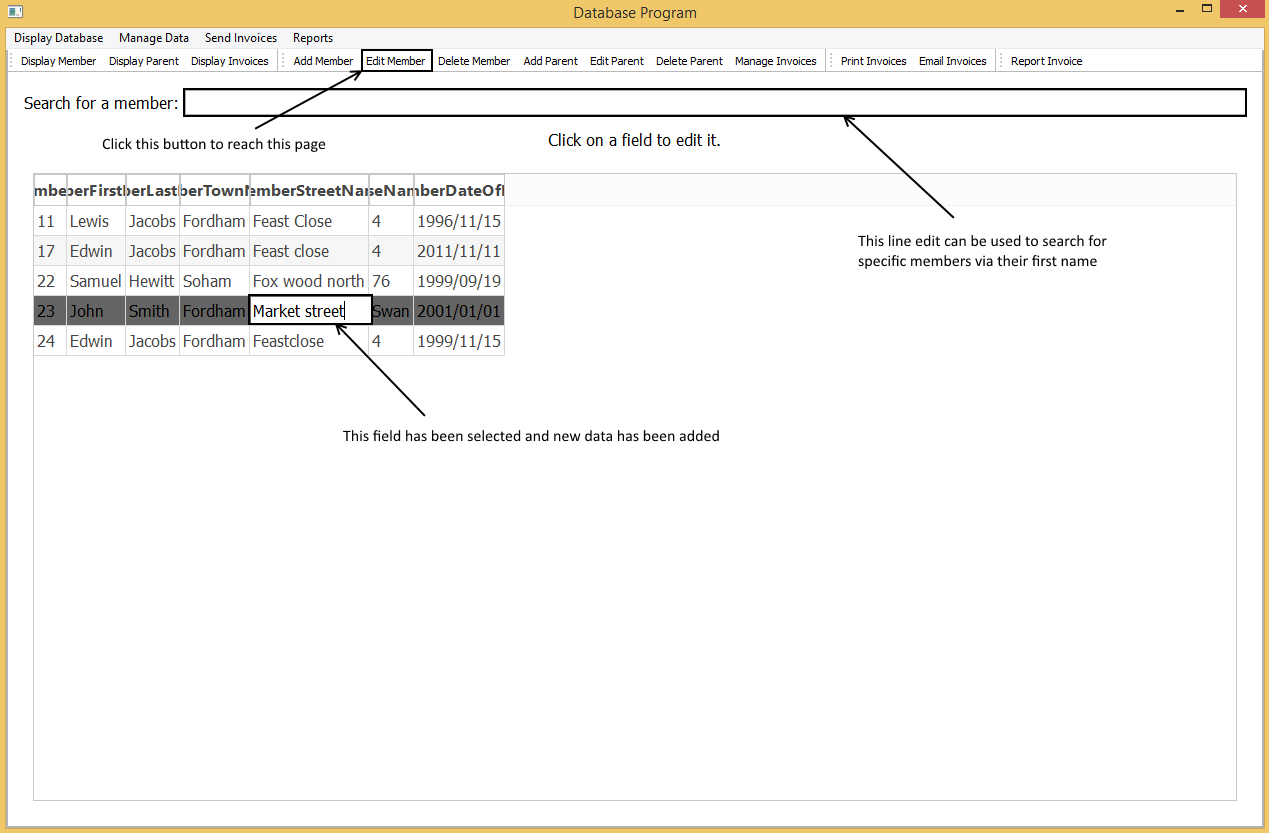
\includegraphics[width=\textwidth]{./Manual/Images/EditMember.png}
	\item To search for a member, enter either the first name or the last name into the box at the top of the page.
	\item To edit a member, click on the field you wish to edit in that member and type the new data.
	\item When done, press enter and the new data will permanently overwrite the old data.
	\item 
\end{enumerate}

\subsubsection{How is a member deleted?}
\label{delete_member}

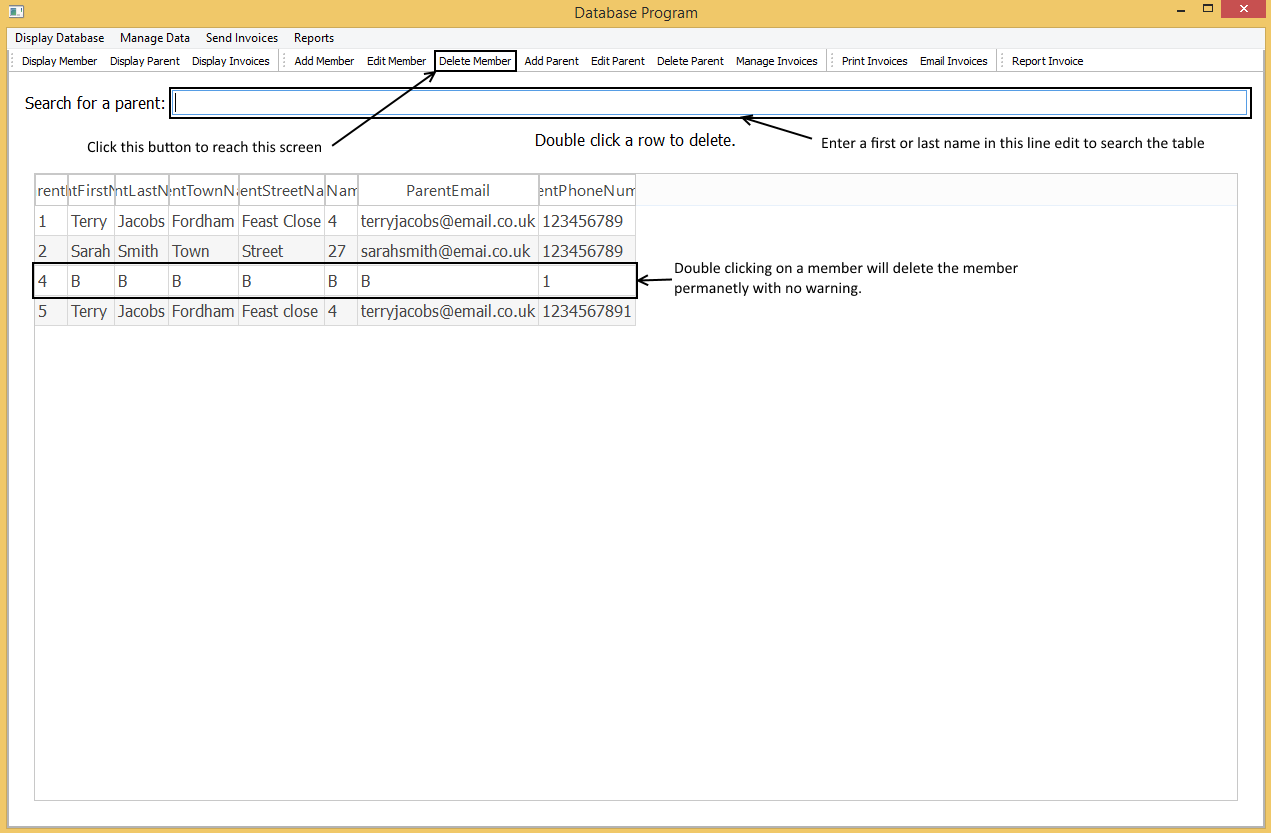
\includegraphics[width=\textwidth]{./Manual/Images/DeleteMember.png}

\begin{enumerate}
	\item Click the Delete Member button on the menu bar in the drop down menu under Manage Data or directly on the tool bar.
	\item 
	\item 
	\item 
	\item 
\end{enumerate}

To show the Delete Member tab, click the Delete Member button on the menu bar in the drop down menu under Manage Data or directly on the tool bar. This screen is used for deleting members by double clicking on the member you wish to delete. The member will be deleted without warning instantly and permanently. To search for a member by first or last name, type the name into the searching line edit.

The deletion of a member cannot be undone!

\subsubsection{How do I show which invoices have not been paid?}
\label{report_invoice}

\begin{enumerate}
	\item 
	\item 
	\item 
	\item 
	\item 
\end{enumerate}

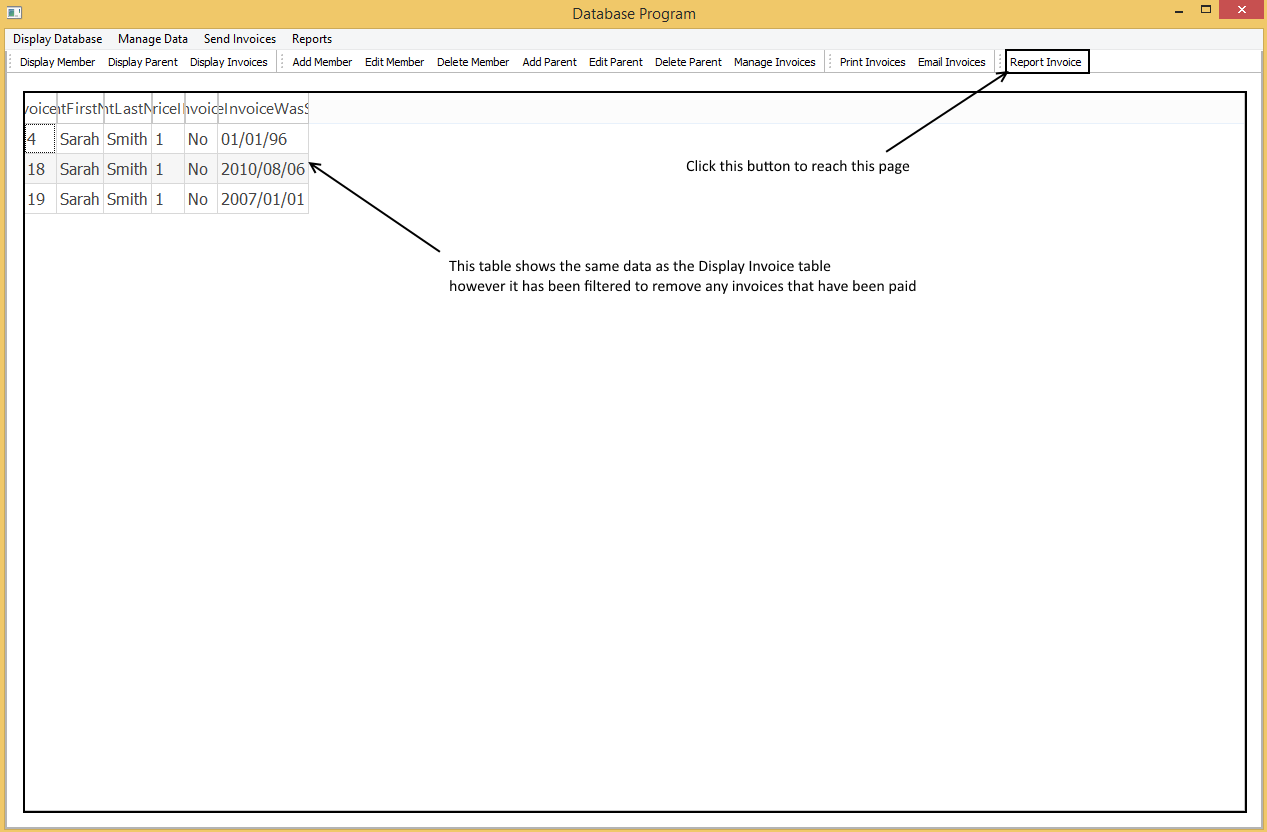
\includegraphics[width=\textwidth]{./Manual/Images/ReportInvoice.png}

To show the Report Member tab, click the Report Member button on the menu bar in the drop down menu under Reports or directly on the tool bar. This screen is used for showing which invoices have not been paid.


\subsection{Saving}
The database is automatically saved every time it is interacted with. This means that whenever any entity is added, edited or deleted the database will permanently be saved. The database cannot be manually saved.

There is no way to backup the database in the program, however copying the file ''scout\_database.db'' is an easy way of backing up the data.

 
\subsection{Limitations}
The system does not email invoices and does not print specific invoices, only a template. This is because I ran out of time during the implementation stage.


\section{Error Recovery}

\subsection{Error with deletion}
There is a major flaw in the program, that the user should be aware of. The flaw is that when an entity is double clicked in any table after accessing any Delete tab that entity will be permanently deleted with no way of recovery. Care must be taken after using the Delete function to not double click any entities, especially when clicking fields when editing.

\begin{figure}[H]
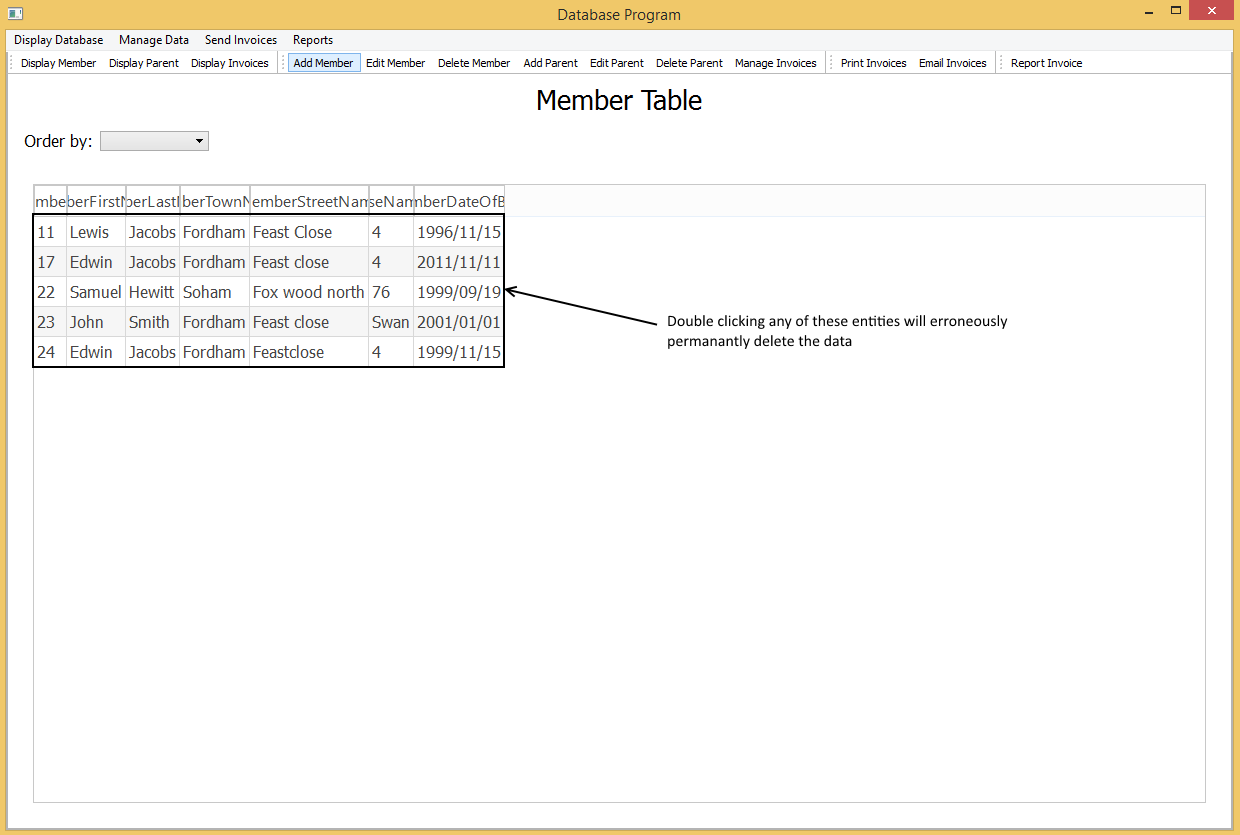
\includegraphics[width=\textwidth]{./Manual/Images/DeleteError.png}
    \caption{Delete Error} \label{fig:delete_error}
\end{figure}

\section{System Recovery}

\subsection{Backing-up Data}

\begin{figure}[H]
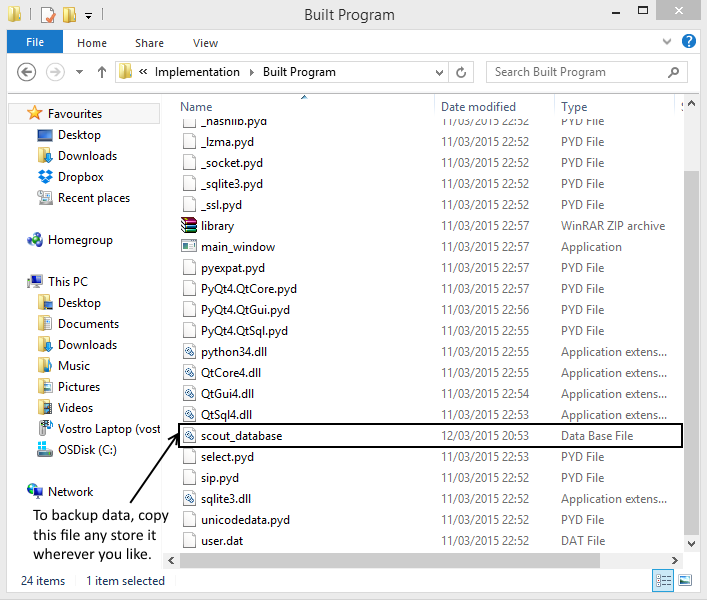
\includegraphics[width=\textwidth]{./Manual/Images/BackupData.png}
    \caption{Backup Data} \label{fig:backup_data}
\end{figure}


To backup the data, simply copy the ''scout\_database'' file, first ensuring that the program is closed.

\subsection{Restoring Data}
The copied file can be copied into the same folder it came out of under the same name to reimplement the data.

\stopcontents[manual]